%%%%%%%%%%%%%%%%%%%%%%%%%%% asme2ej.tex %%%%%%%%%%%%%%%%%%%%%%%%%%%%%%%
% Template for producing ASME-format journal articles using LaTeX    %
% Written by   Harry H. Cheng, Professor and Director                %
%              Integration Engineering Laboratory                    %
%              Department of Mechanical and Aerospace Engineering    %
%              University of California                              %
%              Davis, CA 95616                                       %
%              Tel: (530) 752-5020 (office)                          %
%                   (530) 752-1028 (lab)                             %
%              Fax: (530) 752-4158                                   %
%              Email: hhcheng@ucdavis.edu                            %
%              WWW:   http://iel.ucdavis.edu/people/cheng.html       %
%              May 7, 1994                                           %
% Modified: February 16, 2001 by Harry H. Cheng                      %
% Modified: January  01, 2003 by Geoffrey R. Shiflett                %
% Modified: July 19, 2009 as a template in a single column for       %
%           ASME Journals by Harry H. Cheng                          %
% Use at your own risk, send complaints to /dev/null                 %
%%%%%%%%%%%%%%%%%%%%%%%%%%%%%%%%%%%%%%%%%%%%%%%%%%%%%%%%%%%%%%%%%%%%%%

%%% use 10pt options with the asme2ej format
\documentclass[10pt]{asme2ej}
\usepackage{graphicx}
\graphicspath{{../Images/}}
\usepackage{float}
\usepackage{amsfonts, amsmath, amssymb}

\usepackage{epsfig} %% for loading postscript figures

%% The class has several options
%  onecolumn/twocolumn - format for one or two columns per page
%  10pt/11pt/12pt - use 10, 11, or 12 point font
%  oneside/twoside - format for oneside/twosided printing
%  final/draft - format for final/draft copy
%  cleanfoot - take out copyright info in footer leave page number
%  cleanhead - take out the conference banner on the title page
%  titlepage/notitlepage - put in titlepage or leave out titlepage
%  
%% The default is oneside, onecolumn, 10pt, final


\title{Sampling on High Frequency BTCUSD(T) data}

%%% first author
\author{Christos Koutkos
    \affiliation{
	WQU Student - Researcher,\\
	Master in Math\\ 
	Greece, Zakynthos\\
    Email: christoskoutkos@msn.com
    }	
}

%%% second author
%%% remove the following entry for single author papers
%%% add more entries for additional authors
\author{Tilemachos Kosmetsas
	\affiliation{WQU Student - Researcher,\\
	Mathematician\\
	Greece, Thessaloniki\\
        Email: kosmetsastilemahos@yahoo.com
    }
}

%%% third author
%%% remove the following entry for single author papers
%%% add more entries for additional authors
\author{Third Co-author\\
        Greg Cireci 
    \affiliation{Professor,\\
        WorldQuant University\\
        New York\\
        Email: greg.ciresi@masters.wqu.edu
    }
}


\begin{document}

\maketitle    

%%%%%%%%%%%%%%%%%%%%%%%%%%%%%%%%%%%%%%%%%%%%%%%%%%%%%%%%%%%%%%%%%%%%%%
\begin{abstract}
{\it 
In the past couple of years, a vast inflow of retail and corporate capital has entered
into the cryptocurrency markets. As time goes by, one may notice a rising interest in these
markets, as well as, an almost exponential increase in trading volumes. Although the
cryptocurrency market has many similarities with the traditional well-documented
markets, the authors felt that even the slightest and subtle difference between them, is
enough to differentiate the behavior of assets such as Bitcoin and thus investigation and
research is deemed mandatory. Features such as its volatile nature, along with its many
other special characteristics, constitute Bitcoin, as a speculative and perhaps a hedging
instrument among others. The interest that surrounds this market, has captivated the
authors as well, and thus they decided to study Bitcoin spot and futures timeseries. This
assignment is based on the premise, that there is a fast-growing interest in trading crypto
assets and that there is need for more research on the field. More specifically, it is well
known that high frequency trading requires necessary data handling and most certainly
appropriate sampling, in such a way, that market structure alterations can be captured
and that meaningful signals can be extrapolated.
By researching the BTC timeseries the authors will attempt to sample BTC spot data with the intention of extrapolating the aforementioned signals, and if
possible, information surges (market structure changes).

\textbf{Keywords}: BTCUSD(T), PCA Analysis, metric, sampling, imbalance bars, information,
signal 
}
\end{abstract}




%%%%%%%%%%%%%%%%%%%%%%%%%%%%%%%%%%%%%%%%%%%%%%%%%%%%%%%%%%%%%%%%%%%%%%



\section{Introduction}

\subsection{Problem Statement}

The approach the authors will take in this assignment is to analyze existing ideas and implement them on BTC timeseries, but at the same time, explore new approaches and combinations. The difficulty of this project lies with the asynchronous nature of information.
The way that information appears in the market must dictate the way they are represented, perceived by the researcher and used by a model. To illustrate this, we will use BTCUSD volume data, from Bitstamp exchange with index ranging from 2020-06-15 to 2020-09-15, aggregated weekly.

\begin{figure}[H]
	\centering
	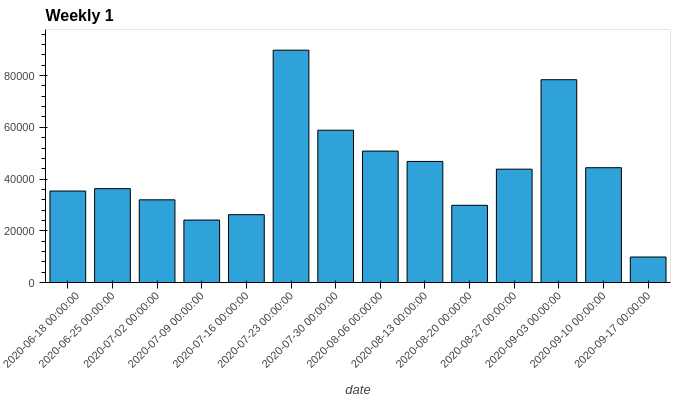
\includegraphics[width=6cm, height = 3.3cm]{one}
	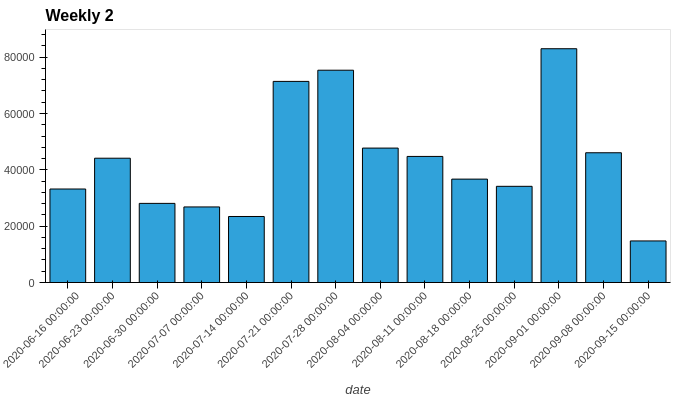
\includegraphics[width=6cm, height = 3.3cm]{two}
	\\[\smallskipamount]
	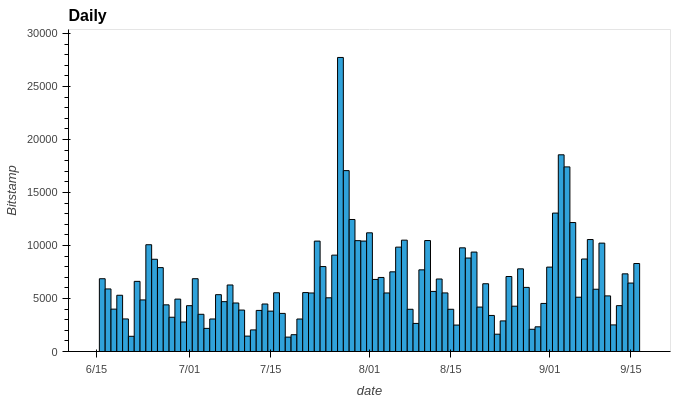
\includegraphics[width=6cm, height = 3.3cm]{three}
	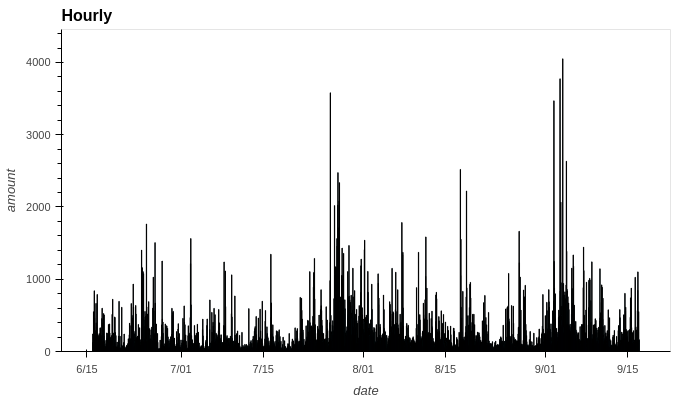
\includegraphics[width=6cm, height = 3.3cm]{four}
	\caption{BTCUSD Volume sampled in several timeframes}\label{fig:example}
\end{figure}

On the \textit{Weekly 1} chart, we observe that the week starting at 2020-07-23, has the biggest spike in volume across these 3 months while the next weeks exhibit declining volume. Another spike at
the week starting at 2020-09-03, also takes place. The \textit{Weekly 2} chart, is drawn on the same data, but before aggregating in weekly
timeframe (from daily), the dataset got shifted by 3 days to the left. As a result, the new chart is different from the previous one, as we observe
that the 2 week period that begins at 2020-07-21 had significant volume, but the highest spike now occurs at the week that starts 2020-09-08.

By changing the resolution to the daily timeframe, we observe that the volume that was attributed to two weeks in the previous graph, actually took place in 5 days, and the biggest spike in volume occurred in 2020-7-25. Further enhancing the resolution and aggregating to the hourly timeframe, the \textit{Hourly} chart,
shows a different story. There is a cluster of volume ocurring at 2020-07-25 and persisting for
the coming week. More importantly, we observe a second spike around 2020-09-05 that is more pronounced but not as persistent (in terms of lags) as the first one.

\begin{figure}[H]
	\centering
	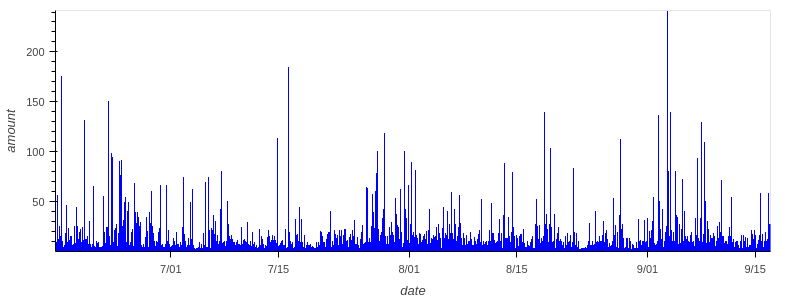
\includegraphics[width=10cm, height = 4cm]{five.png}
	\caption{Volume per trade (tick volume).}
	\label{fig:tick_vol}
\end{figure}

Lastly, graph \ref{fig:tick_vol}, is the highest resolution possible and contains all the information we could possible get for volume in Bitstamp during that period. This chart, looks more like a series of impulses (sudden spikes) while some clusters of volume can be seen on the bottom of the graph. 

What a researcher and an algorithm might extract from the above data, could be different in
each occasion, nevertheless, it is the same data (except for the 3 days shift that illustrate the danger of sampling in large timeframes), containing the same information. The above example used different fixed timeframe intervals but the same applies to sampling based on the side of the trade, or the number of trades. 

So, why not always use the highest resolution possible, in order to preserve all the information? This question leads us to the next tradeoff: The lower the resolution, the more information is lost, and the higher it is, the more noisy and less useful the data become.

The above example illustrates the main drive of this project: the necessity for proper sampling in high frequency data.

%%%%%%%%%%%%%%%%%%%%%%%%%%%%%%%%%%%%%%%%%%%%%%%%%%%%%%%%%%%%%%%%%%%%%%

\subsection{Literature Review}

The goal of this literature review is to identify the “avant garde” of researchers in this
emerging field, to summarize the up-to-date research results regarding data sampling and
pattern recognition and to pinpoint the most cutting-edge results. The authors will then try to
place themselves in this large picture and hopefully contribute to technical analysis and data
sampling family.

The main driver of this project, is Advances in Financial Machine Learning (De Prado
2018). In his book De Prado gives basic insight on how to sample and prepare data. Specifically,
he uses the word “information” in a microstructural sense and proposes the creation of bars,
albeit at an entry level, such as tick imbalance bars, volume/fiat bars and tick run bars. These
bars could potentially produce signals, that are “triggered” when a certain threshold is
exceeded, e.g., a certain amount of volume is being traded, at a certain time, that is beyond the
expected level.

In the third edition of his book Analysis of financial time series (Tsay 2010) chapter 12,
Gibb’s sampling, which is a Markov Chain Monte Carlo method is used. This method enables
statistical inference, and has the advantage of “decomposing a high-dimensional estimation” to
a problem with lower parameter problem. The insight that can be taken from this, is to
approach Bitcoin signal extraction by removing certain correlated features. An in-detail Python
application of the MCMC method is illustrated in the Python for Finance (Yves Hilpisch 2015).

An interesting statistical approach on defining and identifying a “Bull or Bear” market
can be found on the paper: Defining and Dating Bull and Bear Markets: Two Centuries of
evidence. (Gonzalez, Hoang, Powell, Shi 2006). This paper is not cryptocurrency specific but the
way it defines these terms is relevant to Bitcoin. The basic tool for identifying the markets being
used is the persistence of the time-series above or below one or more moving averages
(Turning point methods BB and CC as they are called by the authors).

Another paper published on 2019 called Exogenous Drivers of Bitcoin and
Cryptocurrency Volatility – A mixed Sampling Approach to Forecasting (Walther, Klein , Bouri)
expands on the mixed sampling method (Garch-Midas) regarding volatility of certain
cryptocurrencies during high price movements. This paper in short concludes that exogenous
factors are better suited for predicting high volatilities during Bear markets than say the Garch
model.

Technical Analysis for Algorithmic Pattern Recognition ( Zapranis Tsinaslanidis 2016) is a
book expanding on technical analysis and will be exceptionally useful because it provides insight
on patters: holding, support and resistance levels recognition. It expands on indicators and
tools such as RSI , Bollinger Bands and MA convergence-divergence.


\section{Exploration}

section{Introduction}

In this chapter, we will explore the BTCUSD(T) market across 5 major exchanges by following a visual approach on aggregated data. Our initial sampling approach will be across time (fixed time window). Key insights that will be extracted, will serve as the infrastructure of a dynamic way of sampling. 


\subsection{Volume}

It is commonly accepted that volume is one of the most important tools, for analyzing timeseries in finance. Exploring volume across exchanges is a significant task that will provide our analysis with the insights as to how someone should proceed in using trade-to-trade and aggregated volume in several windows, in order to create meaningful signals.

The trade data for BTCUSD begin as early as 2011, with few exchanges offering the opportunity to trade this asset. The first exchange was MtGox. It was launched in 2010 and shut down in April 2014 due to fraud, as more than 850,000 BTC were missing \cite{wiki_mt}. As time passed by, and BTC gained more traction, the trading volume upscaled significantly and more exchanges, such as Bitstamp, Kraken and Coinbase, appeared. Following 2017, a demographic shift took place: Institutions and retailers, started engaging with the crypto sphere and Bitcoin specifically in growing numbers \cite{med}. This was the period that Bitcoin become “known”.

\begin{figure}[H]
	\centering
	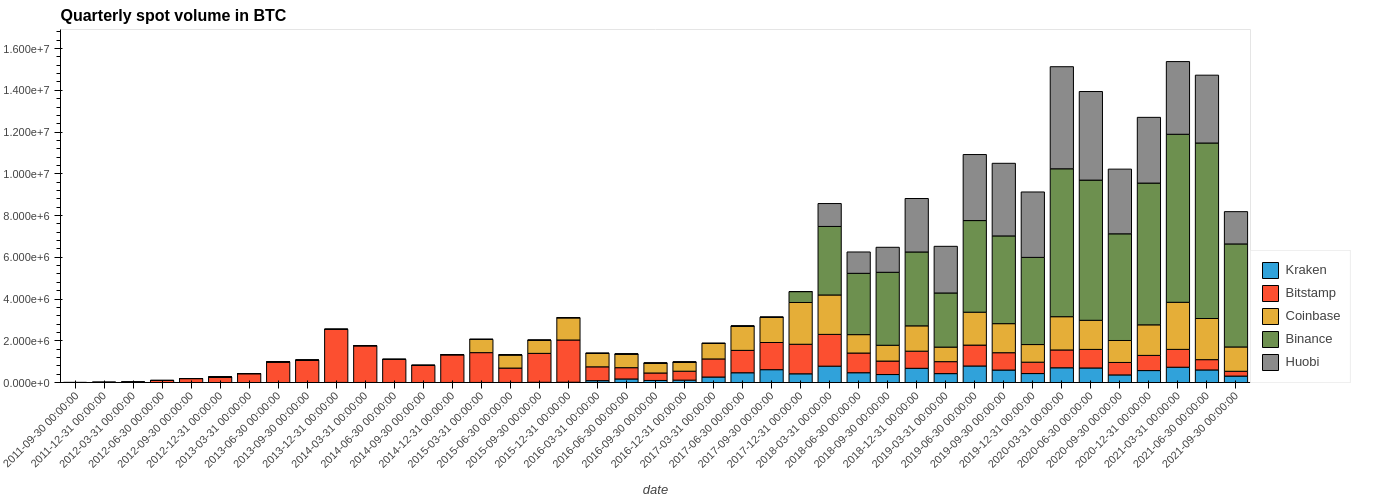
\includegraphics[width=10cm, height = 4cm]{historical_volume.png}
	\caption{Quarterly volume across spot exchanges.}
	\label{fig:hist_vol}
\end{figure}


As we can see in \ref{fig:hist_vol}, the overall trading volume begun to rise in early 2017, as more people were attracted to the impressive BTC bull run, up until that point. At this point, we could distinct the BTCUSD from BTCUSDT volume following the assumption that a retail trader is forced to use fiat currency in order to buy bitcoin for the first time, in some centralized exchange, thus the bitcoin volume on USD, could serve as an indicator of retail activity.


\begin{figure}[H]
	\centering
	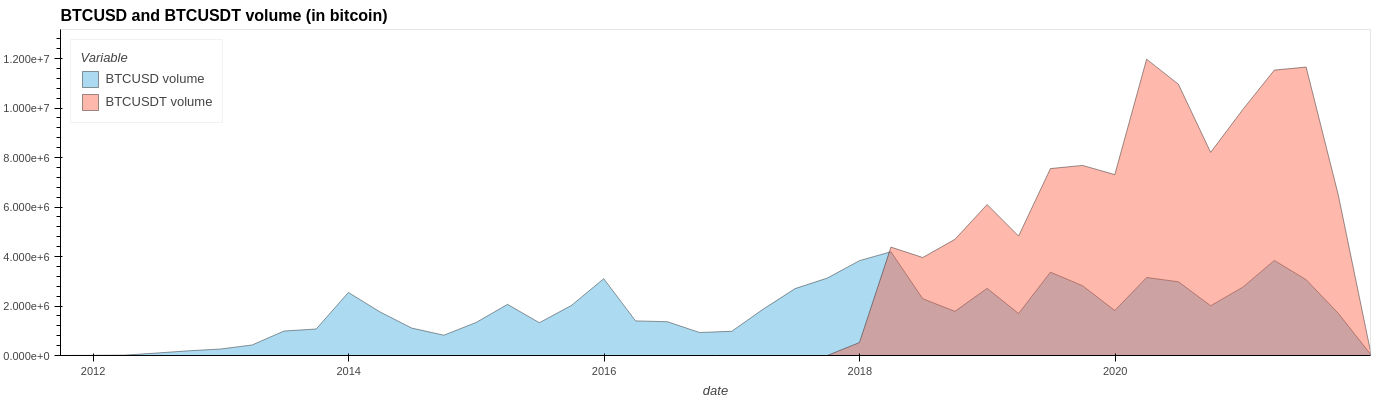
\includegraphics[width=10cm, height = 4cm]{volume2.png}
	\caption{BTCUSD and BTCUSDT spot trading volume (in bitcoin).}
	\label{fig:vol2}
\end{figure}

The first thing to notice in \ref{fig:vol2}, is that since the 2017 BTC bullrun, the BTCUSD volume (in bitcoin) is slightly elevated. Furthermore, since the introduction of USDT, the exchanges that offered BTCUSDT trading, easily surpassed those that offered only BTCUSD. The latter is to be expected, since USDT is 'tethered' to the USD (stable coin offering safety from volatility), while being at the same time easily transferable across exchanges in contrast to fiat. On the other hand, the \ref{fig:vol3} shows a steep increase in dollars traded that can be attributed to the increase in bitcoin price. 

\begin{figure}[H]
	\centering
	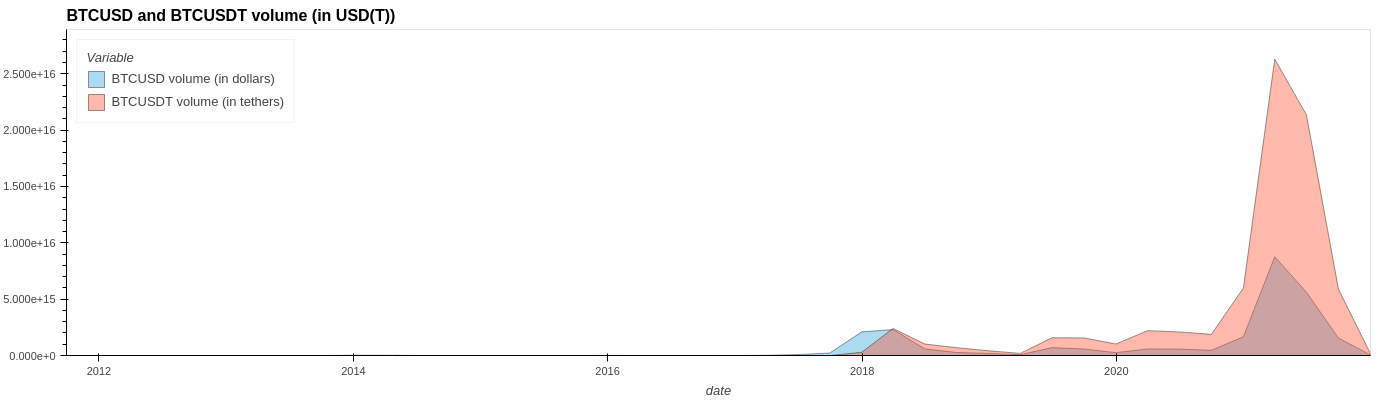
\includegraphics[width=10cm, height = 4cm]{usdusdt.png}
	\caption{BTCUSD and BTCUSDT spot trading volume (in USD(T)).}
	\label{fig:vol3}
\end{figure}

In the next four graphs \ref{fig:mean}, we can see the mean trading volume in bitcoin and dollars for BTCUSD and BTCUSDT. As we expect, in the upper two graphs, the mean trading volume decreases as bitcoin price increases. In contrast to the above, the bottom graphs, show an increase in mean trading volume, although, this increase, is different for the two markets: the BTCUSD market shows the 'anticipated' behavior that can be explained by the BTC price and the increased interest to this new asset, and the BTCUSDT market, exhibits a smaller increase in mean trading volume (dollars) even though the volume traded in USDT is higher than the volume traded in USD. The latter indicates the existence of many small buy/sell orders in the USDT markets.

\begin{figure}[H]
	\centering
	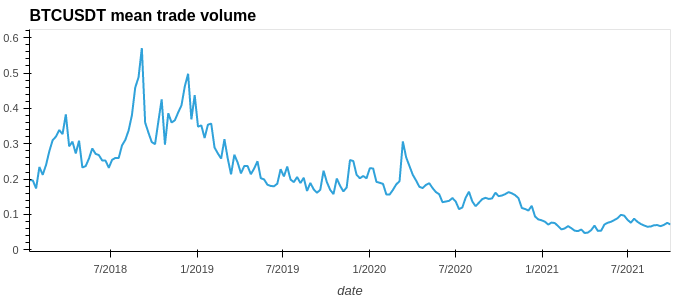
\includegraphics[width=6cm, height = 3.3cm]{mean1}
	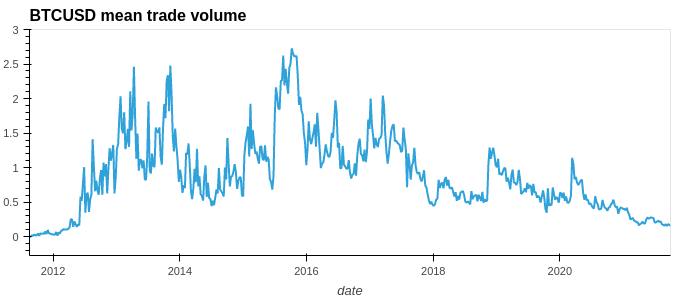
\includegraphics[width=6cm, height = 3.3cm]{mean2}
	\\[\smallskipamount]
	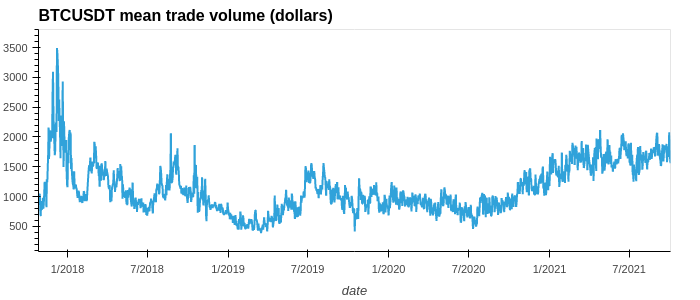
\includegraphics[width=6cm, height = 3.3cm]{mean3}
	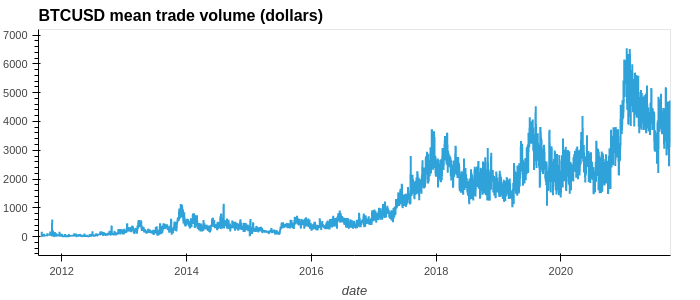
\includegraphics[width=6cm, height = 3.3cm]{mean4}
	\caption{Mean volume per trade.}
	\label{fig:mean}
\end{figure}


An approach that may disclose the “nature” of the investor based on the trade data at hand, would be to use the following framework of assumptions: 
\begin{itemize}
	\item Retail traders are trading in integer dollar volumes, and most likely in multiples of 10, and
	\item Institutional investors will more likely buy and sell in OTC (Over The Counter) markets.
\end{itemize} 

In order to extract the possible retail trades, we chose a mean transaction cost \( c = 0.022\% \) per trade, and extracted it from all trades. If a trade was divisible by 10, it was classified as a retail trade. Nevertheless, the fee structure is different across exchanges and even different across traders in the same exchange (volume per month dependent). Therefore, we chose to include an error \(e = \$0.15 \) as an acceptable distance from the closer mutliple of 10. The trades chosen, should be trades made manually by some trader and not an algorithm (that tends to trade in many decimals). Furthermore, these trades could be made by a professional of a small magnitude and not a retail trader. For briefness purposes, we will refer to these trades, as retail trades, and the traders that initiated them, as retail traders. The above assumptions are flawed in the sense that someone can buy/sell in bitcoin denominated  values (0.5 btc or 1 btc), therefore, this metric can capture only a small percentage of retail trades. Nevertheless, based on the data that the authors possess, there is no other way to classify a trade as 'retail trade'.

In the figure \ref{fig:ret1}, we can see that the estimated number of retail trades on BTCUSDT, is from 4 to 12 times bigger than the one on BTCUSD. Since a retail trader that wishes to trade for the first time, is forced to use fiat currency, we could assume, that the BTCUSDT trades, were executed from retail traders that were active in previous market cycles as well (2017 bull run and before). 

On the top right graph, we can see the ratio of BTCUSDT to BTCUSD trades. We observe that the top is reached during May 2021, when the first large correction of the latest bull markets occured. 



\begin{figure}[H]
	\centering
	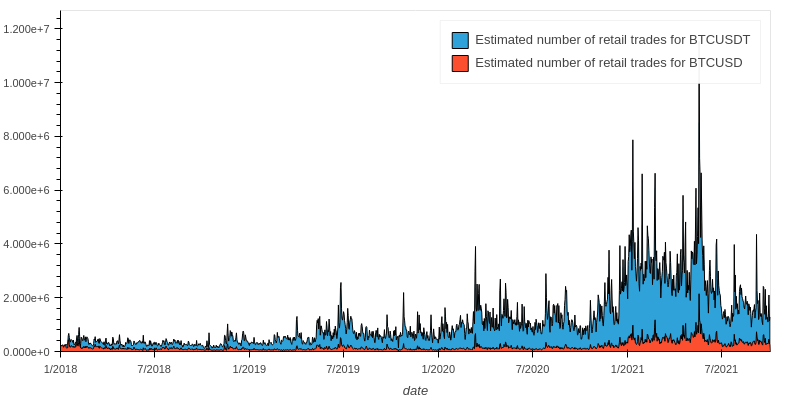
\includegraphics[width=6cm, height = 3.3cm]{ret_trades_1.png}
	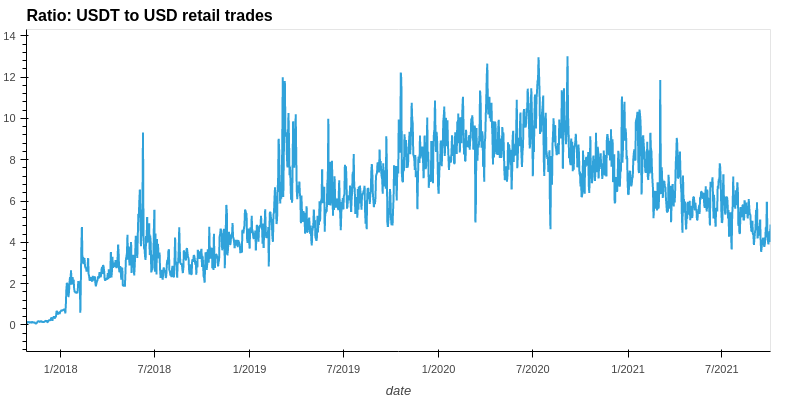
\includegraphics[width=6cm, height = 3.3cm]{ratio_ret_trades.png}
	\\[\smallskipamount]
	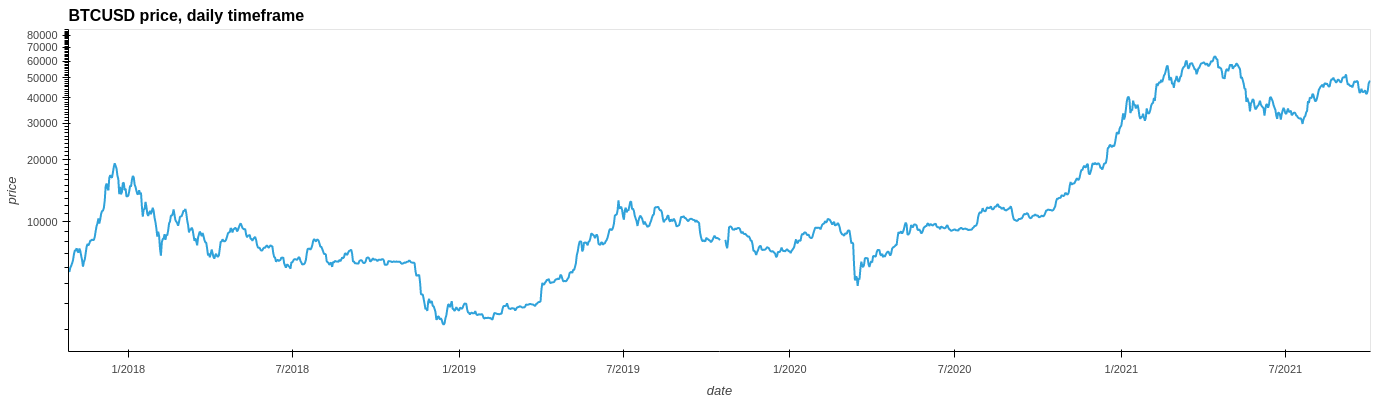
\includegraphics[width=12.2cm, height = 3.3cm]{price_retail.png}
	\caption{Retail trades and BTC price.}
	\label{fig:ret1}
\end{figure}

The increasing ratio indicates that BTCUSDT trades are relatively more precise in following the bull run (experienced retail traders) while the ratio starts declining, close to market top, indicating the timing when retail activity starts to gain traction in BTCUSD market, where is more likely for a 'first time retail trader' to trade.

On the next histograms, the difference in retail activity between BTCUSD and BTCUSDT becomes even more apparent. In the BTCUSD case, the graph is skewed to the left, with few days distributed to the extremes \( > 600,000 \). The BTCUSDT markets though, as indicated from standard deviation which is 3 times greater than the one in BTCUSD, show that the retail activity is distributed more evenly.

\begin{figure}[H]
	\centering
	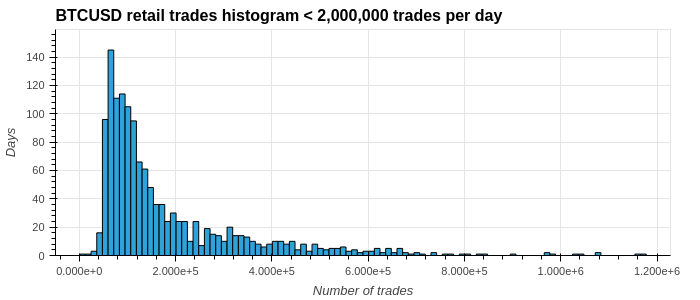
\includegraphics[width=6cm, height = 3.3cm]{btcusd_hist.png}
	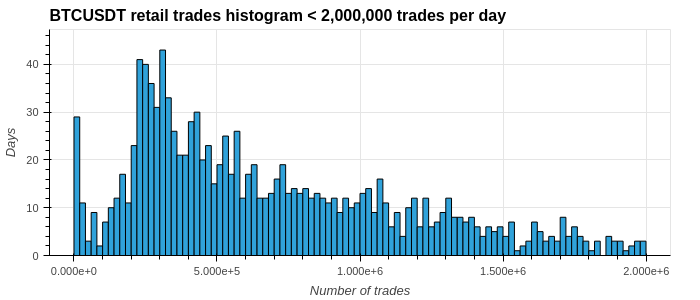
\includegraphics[width=6cm, height = 3.3cm]{btcusdt_hist.png}
	\caption{Histogram of BTCUSD and BTCUSDT no of retail trades per day}
	\label{fig:hist}
\end{figure}

From the summary statistics, we can see that the mean, 25\%, 50\% and 75\% are three to four times greater in BTCUSDT markets, indicative of the preference of retail traders to USDT.


\begin{center}
	\begin{tabular}{ |p{3cm}||p{3cm}|p{3cm}| }
		\hline
		\multicolumn{3}{|c|}{Summary Statistics} \\
		\hline
		& BTCUSD  & BTCUSDT \\
		\hline
		count   & 1.372000e+03	   &1.206000e+03 \\
		mean &   1.837303e+05	  & 6.846854e+05   \\
		std &1.632955e+05 & 4.669768e+05\\
		min    &1.058000e+03 & 4.790000e+02\\
		25\% &   8.008925e+04  & 3.093760e+05\\
		50\% & 1.186430e+05  & 5.595545e+05   \\
		75\% & 2.206602e+05  & 9.985932e+05\\
		\hline
	\end{tabular}
\end{center}


The differences between BTCUSD and BTCUSDT markets, extend to the bitcoin price as well. In the next figure \ref{fig:premium}, we can see that there are arbitrage opportunities between BTCUSD and BTCUSDT markets but not among the markets themselves. These opportunities seem to be available in periods of sudden price movements, and could be accredited to the difference in volume between the two markets. Throughout the 2021 bull market, there was a consistent discrepancy in the fiat premium index.


\begin{figure}[H]
	\centering
	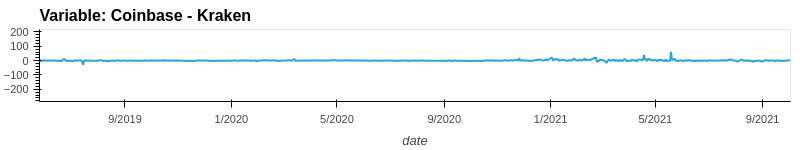
\includegraphics[width=12cm, height = 2.7cm]{pre1.png} \\
	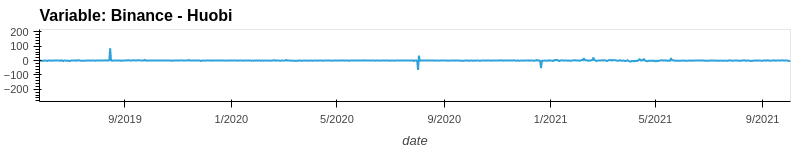
\includegraphics[width=12cm, height = 2.7cm]{pre2.png} \\
	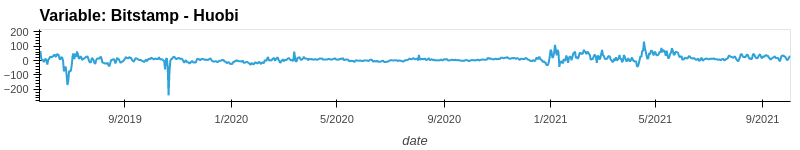
\includegraphics[width=12cm, height = 2.7cm]{pre3.png} \\
	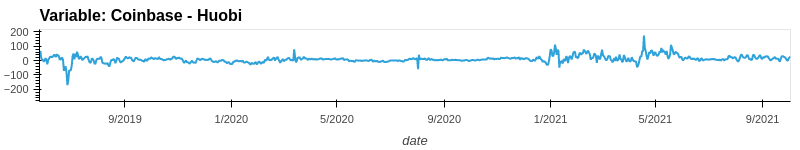
\includegraphics[width=12cm, height = 2.7cm]{pre4.png} \\
	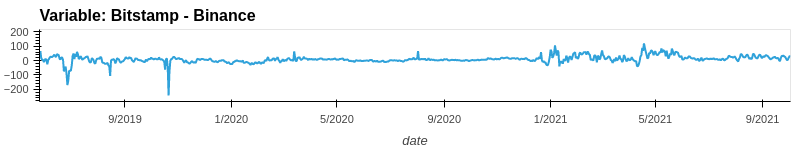
\includegraphics[width=12cm, height = 2.7cm]{pre5.png} \\
	\caption{Fiat premium.}
	\label{fig:premium}
\end{figure}


Such discrepancies could be a valuable source of imbalances, that should be useful for a more precise sampling. Next, we will explore volume, a bit deeper. We will decompose the covariance matrix of volume (eigen decomposition), of the BTCUSD
and BTCUSDT pairs. The computation will take place in a rolling fashion, under a fixed time interval, in order to capture the convergence of volume, between the exchanges and during different phases of the market.


\begin{figure}[H]
	\centering
	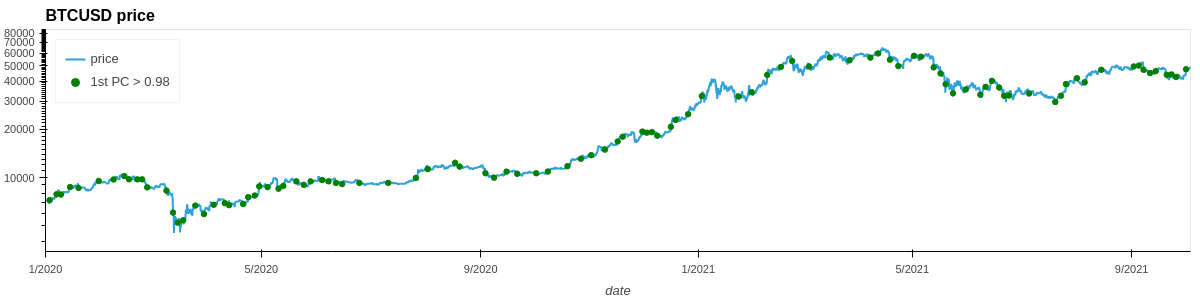
\includegraphics[width=12cm, height = 3cm]{cov1.png} \\
	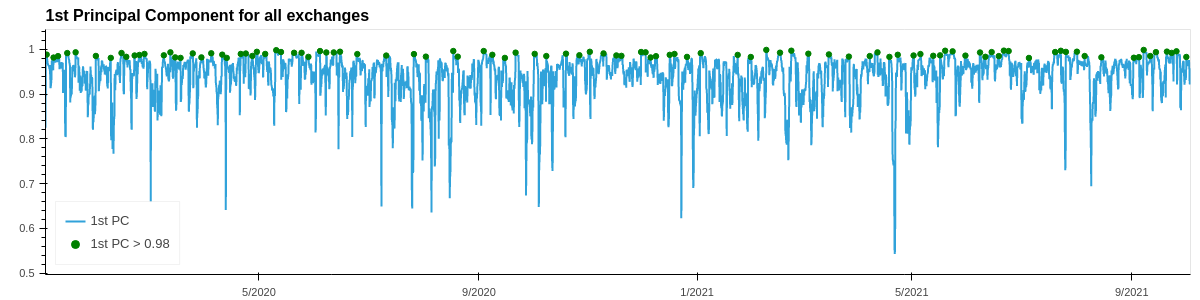
\includegraphics[width=12cm, height = 3cm]{cov2.png} \\
	\caption{PCA analysis - 1st principal component and BTCUSD price.}
	\label{fig:covmatrix}
\end{figure}

In the above figure \ref{fig:covmatrix}, we can see that based on the covariance of the volumes across exchanges, the 1st principal component seems to explain almost all variance, most of the time. This finding, enhances the idea that information is quickly transfered and volumes generally converge. The same must be tested for metrics other than covariance. An appropriate such metric, is the first principal component computed from the eigendecomposition of the Kendall correlation matrix. Since the volumes are not normally distributed (figure \ref{fig:kdevol}), we cannot use neither Pearson or Spearman correlation \cite{kendall}.


\begin{figure}[H]
	\centering
	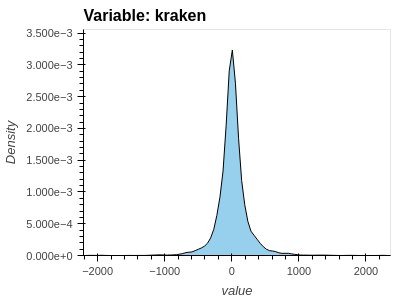
\includegraphics[width=4cm, height = 2.5cm]{kde1.png}
	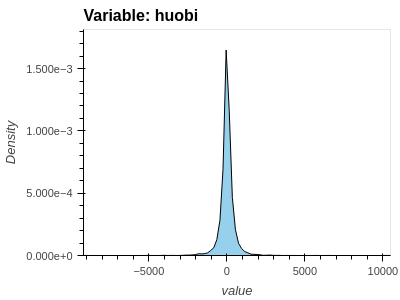
\includegraphics[width=4cm, height = 2.5cm]{kde2.png}
	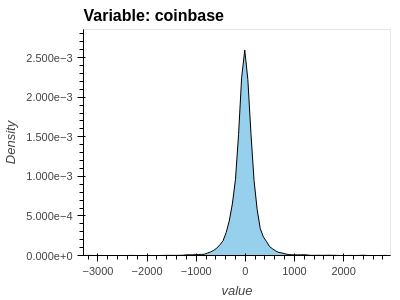
\includegraphics[width=4cm, height = 2.5cm]{kde3.png}
	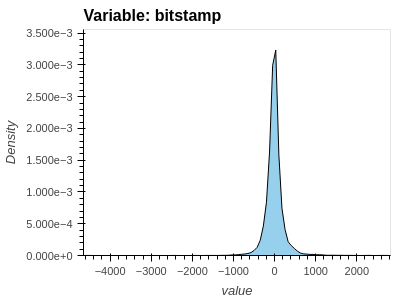
\includegraphics[width=4cm, height = 2.5cm]{kde4.png}
	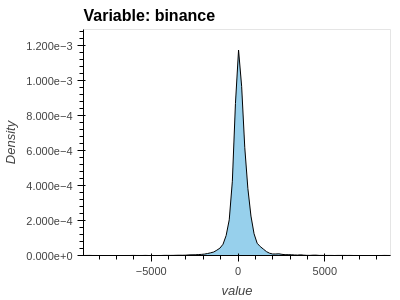
\includegraphics[width=4cm, height = 2.5cm]{kde5.png}
	\caption{KDE plot of volumes aggregated on 4h timeframe, for all exchanges.}
	\label{fig:kdevol}
\end{figure}


Kendall's Tau (\(\tau\)), is a non parametric test that is used to measure the correlation between two variables. There are three different variations of this test, but mostly the Tau-b (\(\tau_b\)) is used. The formula is:
\[
\tau_b = \frac{2(n_c - n_d)}{\sqrt{n(n-1) - G_x}\sqrt{n(n-1) - G_y}} 
\]

where:
\begin{itemize}
	\item \(n_c\) is the number of concordant values
	\item \(n_d\) is the number of discordant values
	\item \(G_{x,y} = \sum{t_i(t_i-1)}\) where \(t_i\) is the number of tied values in the \(i\) group of the \(\{x,y\}\) variable
\end{itemize}

For the following graphs, we need to insert, the notion of positive and negative volumes. The notion of a positive volume (and negative accordingly) is the need to differentiate between the trading volume that leads to positive returns and volume in the market that lead to negative returns. The computations involved the sign of the returns \(b_t = sign\{p_t - p_{t-1}\}\), where \(p_t\) is the price at time \(t\) (this computation took place on tick data therefore \(t\) is the time measured in number of ticks), multiplied with volume at time \(t-1\) : \(b_t \cdot V_{t-1}\). Additionally, by classifying volumes, that inherit a positive or negative sign based on the returns, two sets are formed. 

\begin{figure}[H]
	\centering
	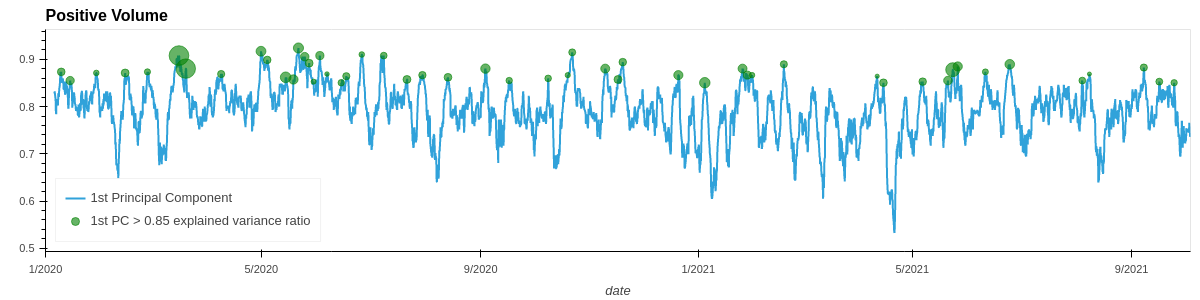
\includegraphics[width=12cm, height = 3.2cm]{kendal4.png} \\
	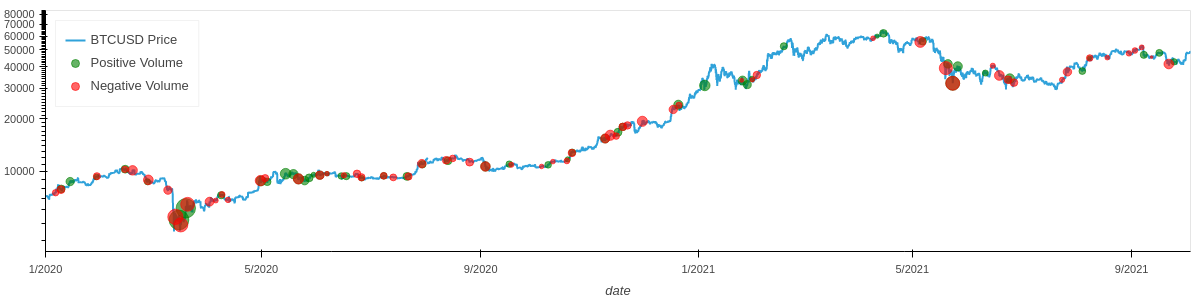
\includegraphics[width=12cm, height = 3.2cm]{kendal3.png} \\ 
	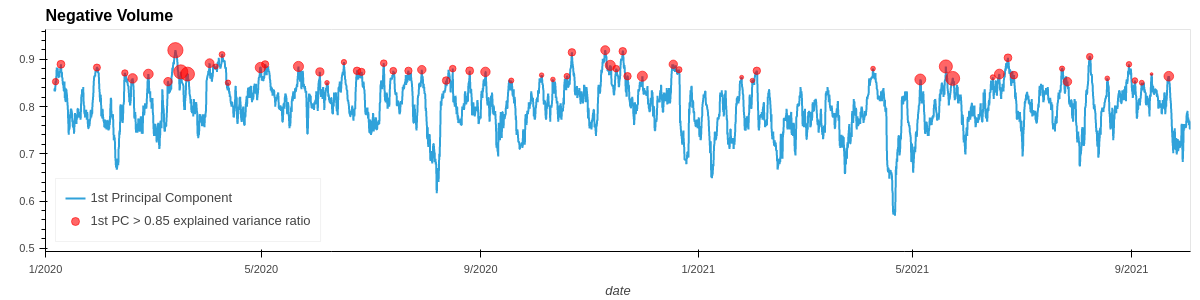
\includegraphics[width=12cm, height = 3.2cm]{kendal1.png} \\
	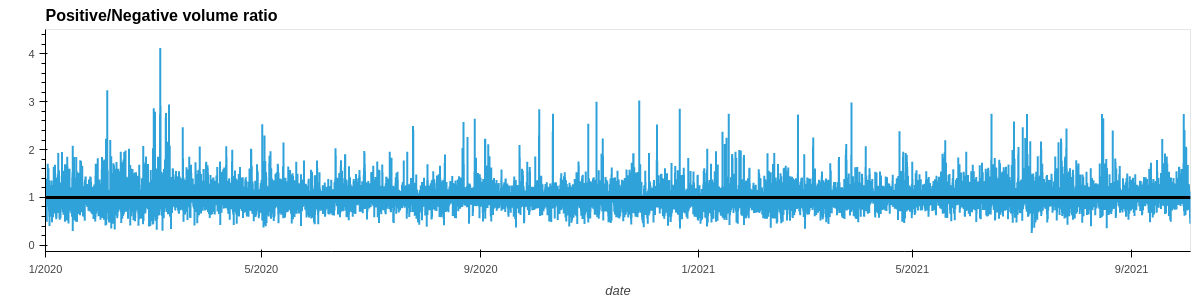
\includegraphics[width=12cm, height = 3.2cm]{kendal2.png} \\
	\caption{Eigendecomposition on kendal correlation matrix for positive and negative volume for \textbf{BTCUSDT} markets.}
	\label{fig:pcakendall}
\end{figure}

In figure \ref{fig:pcakendall} we can see the convergence of positive and negative volumes among BTCUSDT market. The 1st principal component has consistenly high explained variance ratio \( > 0.7 \) which shows that volume between Binance and Huobi, are following the same direction most of the time.

Upon close inspection, it seems that sudden price moves can be associated with higher convergence of volume between the BTCUSDT exchanges. The same seems to be the case, for all exchanges as well (figure \ref{fig:covmatrix}). That leads us to the idea that we could sample when there is convergence in a feature of choice (volume, positive-negative volume, buy/sell volume, number of trades per interval), assuming that in order for such an event to occur, there must be some new information. 

Next, we visualize the number of trades that take place in each exchange. In the figure \ref{fig:nooftrades}, we can see the number of trades aggregated in daily timeframe with the upper chard being in logarithmic scale. We observe that the USDT market is processing many more trades than the USD market. By calculating and comparing the mean number of trades per exchange across 2020 and 2021, we find that the mean trades per day of Binance is 5.5 time the mean of Coinbase, 32 times the mean of Kraken and approximately 37 times the mean of Bitstamp. We also observe that the number of trades (aggregated) is presented in waves, with visible spikes around significant price action. Again, these spikes, converge across all exchanges.  

\begin{figure}[H]
	\centering
	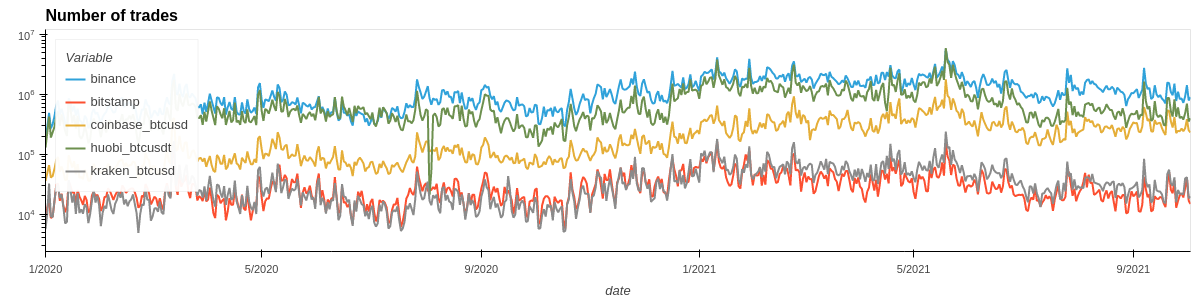
\includegraphics[width=12cm, height = 2.8cm]{No_of_trades_all2.png} \\
	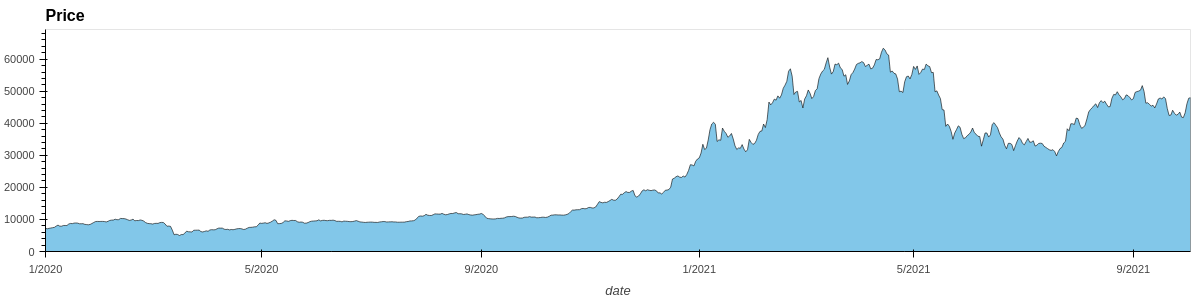
\includegraphics[width=12cm, height = 2.8cm]{No_of_trades_all1.png} \\ 
	\caption{The number of trades aggregated daily, for each exchange. Note that the upper chart is logarithmic.}
	\label{fig:nooftrades}
\end{figure}

In the next figure \ref{fig:nooftrades2}, we are separating the bid, from the offer trades, depending on who initiated each trade(based on  dataset labels buy-sell). First thing to notice is that our data is corrupted, since for approximately 15 days, all trades are classified as trades, initiated by buyers. Due to this shortcoming, in any attempt to use the side of the trade (bid-offer), we will have to exclude this portion of the dataset. Furthermore, the Binance, as expected, processes the largest amount of orders, either buying or selling, but in several spikes, Huobi seems to catch or even suprass Binance. Last but not least, it is interesting that the amount of trades in Coinbase's BTCUSD pair, are steadily increasing, catching up those of the BTCUSDT market.

\begin{figure}[H]
	\centering
	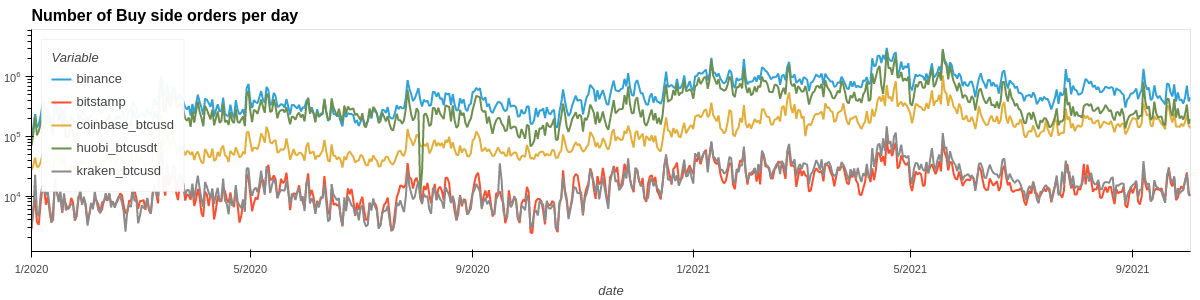
\includegraphics[width=12cm, height = 2.8cm]{nosell1.png} \\
	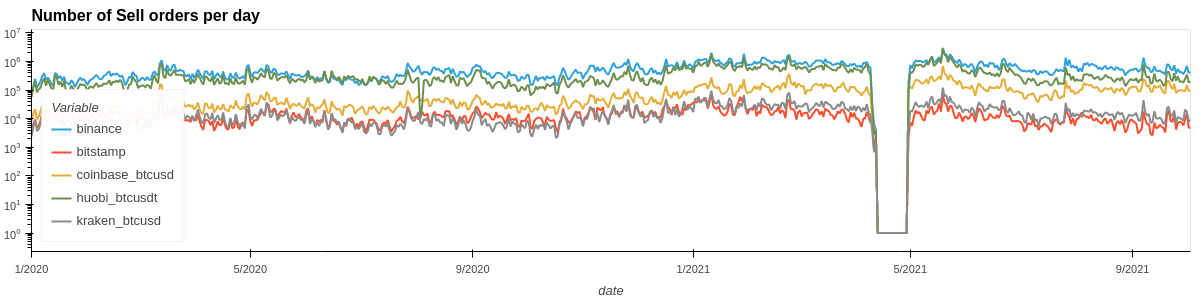
\includegraphics[width=12cm, height = 2.8cm]{nosell2.png} \\ 
	\caption{The number of buy and sell trades aggregated daily, for each exchange. Both charts are logarithmic.}
	\label{fig:nooftrades2}
\end{figure}


The next upper graph \ref{fig:cum}, is produced by taking the cumulative sums of buy side and sell side orders across all exchanges, and subtracting one from the other: 
\[ \text{cumsum}\{\text{Vol}_{\text{Buying}} - \text{Vol}_{\text{Selling}}\} \]
Just before the major bull run of 2020-2021, the selling volume, by far surpassed the buying volume, indicative of the uncertainty of that period (Covid19). Around October 2020, the cumulative sell volume peaked, as shown in the minimum of the graph. From then and on, the buy volume was steadily increasing, which coincides with the price action, at the beginning of the 2020-2021 bull run.  

The second graph is produced by taking the cumsum of the difference of buy and sell volume, but for each exchange individually. An interesting finding is that coinbase and bitstamp are processing more buy side volume than sell side, and more buy volume than any other exchange. The exact opposite is true for Binance, where sell volume is the highest. That alligns with our prior findings, in that BTCUSD market is the entrance of the 'first time' bitcoin buyer, who is attracted during the bull run. 


\begin{figure}[H]
	\centering
	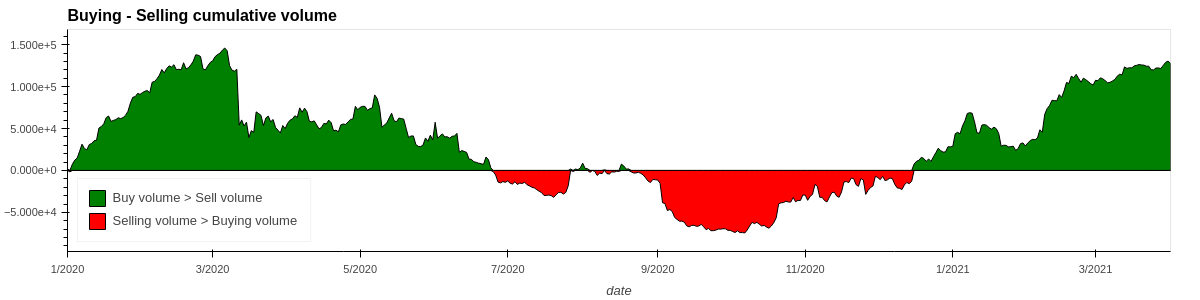
\includegraphics[width=12cm, height = 2.8cm]{buy-sell.png} \\
	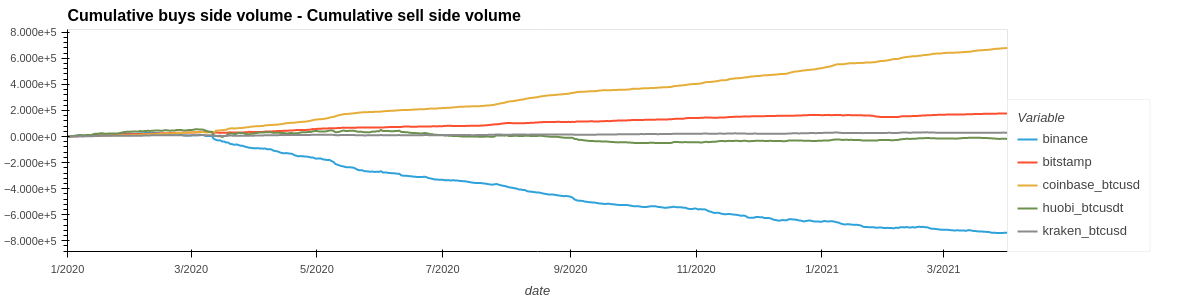
\includegraphics[width=12cm, height = 2.8cm]{cumdif.png} \\ 
	\caption{The number of buy and sell trades aggregated daily, for each exchange. Both charts are logarithmic.}
	\label{fig:cum}
\end{figure}


This discrepancy makes it clear, that even though each exchange has its own pool of
trades, the market dynamics are such, that one needs to consider each exchange not
only individually, but as a single identity as well with a unified liquidity pool. It appears from data, that it is possible that a single exchange can at times attract buyers and on the other hand, another one can attract sellers.
Such a behavior, can be explained by the simplicity of 
transferring tokens between exchanges (e.g. for arbitrage reasons). Especially USDT, XRP,
XLM and DOGE amongst others, seem to have viable liquidity, and very low
transaction finality times and fees. Coins such these, are prime candidates for transferring value fast and cheap.

%%%%%%%%%%%%%%%%%%%%%%%%%%%%%%%%%%%%%%%%%%%%%%%%%%%%%%%%%%%%%%%%%%%%%%





%%%%%%%%%%%%%%%%%%%%%%%%%%%%%%%%%%%%%%%%%%%%%%%%%%%%%%%%%%%%%%%%%%%%%%
\section{Use of SI Units}

An ASME paper should use SI units.  When preference is given to SI units, the U.S. customary units may be given in parentheses or omitted. When U.S. customary units are given preference, the SI equivalent {\em shall} be provided in parentheses or in a supplementary table. 

%%%%%%%%%%%%%%%%%%%%%%%%%%%%%%%%%%%%%%%%%%%%%%%%%%%%%%%%%%%%%%%%%%%%%%
\section{Footnotes\protect\footnotemark}
\footnotetext{Examine the input file, asme2ej.tex, to see how a footnote is given in a head.}

Footnotes are referenced with superscript numerals and are numbered consecutively from 1 to the end of the paper\footnote{Avoid footnotes if at all possible.}. Footnotes should appear at the bottom of the column in which they are referenced.


%%%%%%%%%%%%%%%%%%%%%%%%%%%%%%%%%%%%%%%%%%%%%%%%%%%%%%%%%%%%%%%%%%%%%%
\section{Mathematics}

Equations should be numbered consecutively beginning with (1) to the end of the paper, including any appendices.  The number should be enclosed in parentheses and set flush right in the column on the same line as the equation.  An extra line of space should be left above and below a displayed equation or formula. \LaTeX\ can automatically keep track of equation numbers in the paper and format almost any equation imaginable. An example is shown in Eqn.~(\ref{eq_ASME}). The number of a referenced equation in the text should be preceded by Eqn.\ unless the reference starts a sentence in which case Eqn.\ should be expanded to Equation.

\begin{equation}
f(t) = \int_{0_+}^t F(t) dt + \frac{d g(t)}{d t}
\label{eq_ASME}
\end{equation}

%%%%%%%%%%%%%%%%%%%%%%%%%%%%%%%%%%%%%%%%%%%%%%%%%%%%%%%%%%%%%%%%%%%%%%
\section{Figures}
\label{sect_figure}

All figures should be positioned at the top of the page where possible.  All figures should be numbered consecutively and centered under the figure as shown in Fig.~\ref{figure_ASME}. All text within the figure should be no smaller than 7~pt. There should be a minimum two line spaces between figures and text. The number of a referenced figure or table in the text should be preceded by Fig.\ or Tab.\ respectively unless the reference starts a sentence in which case Fig.\ or Tab.\ should be expanded to Figure or Table.


%%%%%%%%%%%%%%%%%%%%%%%%%%%%%%%%%%%%%%%%%%%%%%%%%%%%%%%%%%%%%%%%%%%%%%
%%%%%%%%%%%%%%%% begin figure %%%%%%%%%%%%%%%%%%%
\begin{figure}[t]
\begin{center}
\setlength{\unitlength}{0.012500in}%
\begin{picture}(115,35)(255,545)
\thicklines
\put(255,545){\framebox(115,35){}}
\put(275,560){Beautiful Figure}
\end{picture}
\end{center}
\caption{The caption of a single sentence does not have period at the end}
\label{figure_ASME} 
\end{figure}
%%%%%%%%%%%%%%%% end figure %%%%%%%%%%%%%%%%%%% 
%%%%%%%%%%%%%%%%%%%%%%%%%%%%%%%%%%%%%%%%%%%%%%%%%%%%%%%%%%%%%%%%%%%%%%

In the following subsections, I have inserted figures that have been provided by authors in order to demonstrate what to avoid.  In each case the authors provided figures that are 3.25in wide and 600dpi in the .tif graphics format.  The papers containing these figures have been held from production due to their poor quality. 

%%%%%%%%%%%%%%%%%%%%%%%%%%%%%%%%%%%%%%%%%%%%%%%%%%%%%%%%%%%%%%%%%%%%%%
\subsection{The 1st Example of Bad Figure}

%%%%%%%%%%%%%%%% begin figure %%%%%%%%%%%%%%%%%%%
%%% 3.34in is the maximum width you can have for a figure
\begin{figure} 
\centerline{\psfig{figure=figure/FMANU_MD_05_1107_11.png,width=3.34in}}
\caption{Example taken from a paper that was held from production because the image quality is poor.  ASME sets figures captions in 8pt, Helvetica Bold.}
\label{fig_example1.ps}
\end{figure}
%%%%%%%%%%%%%%%% end figure %%%%%%%%%%%%%%%%%%%


 
Figurewas taken from a recent paper that was held from publication, because the text is fuzzy and unreadable.  It was probably obtained by taking a screen shot of the computer output of the  software.  This means the original figure was 72dpi (dots per inch) on a computer screen.  There is no way to improve the quality such a low resolution figure.
 
In order to understand how poor the quality of this figure is, please zoom in slightly, say to 200\%.  Notice that while the font of the paper is clear at this size, the font in the figures is fuzzy and blurred.  It is impossible to make out the small symbol beside the numbers along the abscissa of the graph.  Now consider the labels  They are clearly in fonts larger that the text of the article, yet the pixilation or rasterization, associated with low resolution is obvious. This figure must be regenerated at higher resolution to ensure quality presentation.

The poor quality of this figure is immediately obvious on the printed page, and reduces the impact of the research contribution of the paper, and in fact detracts from the perceived quality of the journal itself.



%%%%%%%%%%%%%%%%%%%%%%%%%%%%%%%%%%%%%%%%%%%%%%%%%%%%%%%%%%%%%%%%%%%%%%
\subsection{The 2nd Example of Bad Figure}

%%%%%%%%%%%%%%%% begin figure %%%%%%%%%%%%%%%%%%%
\begin{figure} 
\centerline{\psfig{figure=figure/FMANU_MD_05_1272_5.png,width=3.34in}}
\caption{While this figures is easily readable at a double column width of 6.5in, when it is shrunk to 3.25in column width the text is unreadable.   This paper was held from production.}
\label{fig_example2.ps}
\end{figure}
%%%%%%%%%%%%%%%% end figure %%%%%%%%%%%%%%%%%%%

Figure~\ref{fig_example2.ps}
demonstrates a common problem that arises when a figure is scaled down fit a single column width of 3.25in.  The original figure had labels that were readable at full size, but become unreadable when scaled to half size.  This figure also suffers from poor resolution as is seen in the jagged lines the ovals that form the chain.

This problem can be addressed by increasing the size of the figure to a double column width of 6.5in, so the text is readable.  But this will not improve the line pixilation, and a large low resolution figure is less desirable than a small one.  This also significantly expands the length of the paper, and may cause it to exceed the JMD nine page limit.  Additional pages require page charges of \$200 per page.  It is best to regenerate the figure at the resolution that ensures a quality presentation.


%%%%%%%%%%%%%%%%%%%%%%%%%%%%%%%%%%%%%%%%%%%%%%%%%%%%%%%%%%%%%%%%%%%%%%
\subsection{The 3rd Example of Bad Figure}
%%%%%%%%%%%%%%%% begin figure %%%%%%%%%%%%%%%%%%%
\begin{figure} 
%\centerline{\psfig{figure=figure/FMANU_MD_04_1274_13.ps,width=3.34in}}
\centerline{\psfig{figure=figure/FMANU_MD_04_1274_13.png,width=3.25in}}
\caption{Another example of a figure with unreadable text.  Even when the paper was expanded to double column width the text as shown in Fig.~\ref{fig_example4.ps} was of such low quality that the paper was held from production.}
\label{fig_example3.ps}
\end{figure}
%%%%%%%%%%%%%%%% end figure %%%%%%%%%%%%%%%%%%%

%%%%%%%%%%%%%%%% begin figure %%%%%%%%%%%%%%%%%%%
%%% the maximum width in double column is 6.85in
\begin{figure*} 
\centerline{\psfig{figure=figure/FMANU_MD_04_1274_13.png,width=6.85in}}
\caption{A figure expanded to double column width the text from Figure~\ref{fig_example3.ps}}
\label{fig_example4.ps}
\end{figure*}
%%%%%%%%%%%%%%%% end figure %%%%%%%%%%%%%%%%%%%
An author provided the high resolution image 
in Fig.~\ref{fig_example3.ps}
that was sized to a single column width of 3.25in.  Upon seeing the poor quality of the text, the publisher scaled the image to double column width as shown in Fig.~\ref{fig_example4.ps} 
at which point it took half of a page.  The publisher went on to do this for all eight figures generating four pages of figures that the author did not expect. ASME stopped production of the paper even with the larger figures due to the pixilation of the font.

Clearly the text in this figure is unreadable, and it is doubtful that the author can print the output in a way that it is readable.  This is a problem that the author must solve, not the publisher. 

As you might expect, I have many more examples, but in the end the author is the best judge of what is needed in each figure.  ASME simply requires that the image meet a minimum standard for font and line quality, specifically the font should be the appropriate size and not be blurred or pixilated, and that lines should be the appropriate weight and have minimal, preferably no, pixilation or rasterization.


%%%%%%%%%%%%%%%%%%%%%%%%%%%%%%%%%%%%%%%%%%%%%%%%%%%%%%%%%%%%%%%%%%%%%%
\section{Tables}

%%%%%%%%%%%%%%%%%%%%%%%%%%%%%%%%%%%%%%%%%%%%%%%%%%%%%%%%%%%%%%%%%%%%%%
%%%%%%%%%%%%%%% begin table   %%%%%%%%%%%%%%%%%%%%%%%%%%
\begin{table}[t]
\caption{Figure and table captions do not end with a period}
\begin{center}
\label{table_ASME}
\begin{tabular}{c l l}
& & \\ % put some space after the caption
\hline
Example & Time & Cost \\
\hline
1 & 12.5 & \$1,000 \\
2 & 24 & \$2,000 \\
\hline
\end{tabular}
\end{center}
\end{table}
%%%%%%%%%%%%%%%% end table %%%%%%%%%%%%%%%%%%% 
%%%%%%%%%%%%%%%%%%%%%%%%%%%%%%%%%%%%%%%%%%%%%%%%%%%%%%%%%%%%%%%%%%%%%%

All tables should be numbered consecutively  and centered above the table as shown in Table~\ref{table_ASME}. The body of the table should be no smaller than 7 pt.  There should be a minimum two line spaces between tables and text.


%%%%%%%%%%%%%%%%%%%%%%%%%%%%%%%%%%%%%%%%%%%%%%%%%%%%%%%%%%%%%%%%%%%%%%
\section{Citing References}

%%%%%%%%%%%%%%%%%%%%%%%%%%%%%%%%%%%%%%%%%%%%%%%%%%%%%%%%%%%%%%%%%%%%%%
The ASME reference format is defined in the authors kit provided by the ASME.  The format is:

\begin{quotation}
{\em Text Citation}. Within the text, references should be cited in  numerical order according to their order of appearance.  The numbered reference citation should be enclosed in brackets.
\end{quotation}

The references must appear in the paper in the order that they were cited.  In addition, multiple citations (3 or more in the same brackets) must appear as a `` [1-3]''.  A complete definition of the ASME reference format can be found in the  ASME manual \cite{asmemanual}.

The bibliography style required by the ASME is unsorted with entries appearing in the order in which the citations appear. If that were the only specification, the standard {\sc Bib}\TeX\ unsrt bibliography style could be used. Unfortunately, the bibliography style required by the ASME has additional requirements (last name followed by first name, periodical volume in boldface, periodical number inside parentheses, etc.) that are not part of the unsrt style. Therefore, to get ASME bibliography formatting, you must use the \verb+asmems4.bst+ bibliography style file with {\sc Bib}\TeX. This file is not part of the standard BibTeX distribution so you'll need to place the file someplace where LaTeX can find it (one possibility is in the same location as the file being typeset).

With \LaTeX/{\sc Bib}\TeX, \LaTeX\ uses the citation format set by the class file and writes the citation information into the .aux file associated with the \LaTeX\ source. {\sc Bib}\TeX\ reads the .aux file and matches the citations to the entries in the bibliographic data base file specified in the \LaTeX\ source file by the \verb+\bibliography+ command. {\sc Bib}\TeX\ then writes the bibliography in accordance with the rules in the bibliography .bst style file to a .bbl file which \LaTeX\ merges with the source text.  A good description of the use of {\sc Bib}\TeX\ can be found in \cite{latex, goosens} (see how two references are handled?).  The following is an example of how three or more references \cite{latex, asmemanual,  goosens} show up using the \verb+asmems4.bst+ bibliography style file in conjunction with the \verb+asme2ej.cls+ class file. Here are some more \cite{art, blt, ibk, icn, ips, mts, mis, pro, pts, trt, upd} which can be used to describe almost any sort of reference.

%%%%%%%%%%%%%%%%%%%%%%%%%%%%%%%%%%%%%%%%%%%%%%%%%%%%%%%%%%%%%%%%%%%%%%
\section{Conclusions}
The only way to ensure that your figures are presented in the ASME Journal of Mechanical Design in the way you feel is appropriate and meets the requirement for quality presentation is for you to prepare a double column version of the paper in a form similar to that used by the Journal.

This gives you the opportunity to ensure that the figures are sized appropriately, in particular that the labels are readable and match the size of the text in the journal, and that the line weights and resolutions have no pixilation or rasterization.  Poor quality figures are immediately obvious on the printed page, and this detracts from the perceived quality of the journal.

I am pleased to provide advice on how to improve any figure, but this effort must start with a two-column version of the manuscript. Thank you in advance for your patience with this effort, it will ensure quality presentation of your research contributions.



%%%%%%%%%%%%%%%%%%%%%%%%%%%%%%%%%%%%%%%%%%%%%%%%%%%%%%%%%%%%%%%%%%%%%%
\section{Discussions}
This template is not yet ASME journal paper format compliant at this point.
More specifically, the following features are not ASME format compliant.
\begin{enumerate}
\item
The format for the title, author, and abstract in the cover page.
\item
The font for title should be 24 pt Helvetica bold.
\end{enumerate}

\noindent
If you can help to fix these problems, please send us an updated template.
If you know there is any other non-compliant item, please let us know.
We will add it to the above list.
With your help, we shall make this template 
compliant to the ASME journal paper format.


%%%%%%%%%%%%%%%%%%%%%%%%%%%%%%%%%%%%%%%%%%%%%%%%%%%%%%%%%%%%%%%%%%%%%%
\begin{acknowledgment}
ASME Technical Publications provided the format specifications for the Journal of Mechanical Design, though they are not easy to reproduce.  It is their commitment to ensuring quality figures in every issue of JMD that motivates this effort to have authors review the presentation of their figures.  

Thanks go to D. E. Knuth and L. Lamport for developing the wonderful word processing software packages \TeX\ and \LaTeX. We would like to thank Ken Sprott, Kirk van Katwyk, and Matt Campbell for fixing bugs in the ASME style file \verb+asme2ej.cls+, and Geoff Shiflett for creating 
ASME bibliography stype file \verb+asmems4.bst+.
\end{acknowledgment}

%%%%%%%%%%%%%%%%%%%%%%%%%%%%%%%%%%%%%%%%%%%%%%%%%%%%%%%%%%%%%%%%%%%%%%
% The bibliography is stored in an external database file
% in the BibTeX format (file_name.bib).  The bibliography is
% created by the following command and it will appear in this
% position in the document. You may, of course, create your
% own bibliography by using thebibliography environment as in
%
% \begin{thebibliography}{12}
% ...
% \bibitem{itemreference} D. E. Knudsen.
% {\em 1966 World Bnus Almanac.}
% {Permafrost Press, Novosibirsk.}
% ...
% \end{thebibliography}

% Here's where you specify the bibliography style file.
% The full file name for the bibliography style file 
% used for an ASME paper is asmems4.bst.
\bibliographystyle{asmems4}

% Here's where you specify the bibliography database file.
% The full file name of the bibliography database for this
% article is asme2e.bib. The name for your database is up
% to you.
\bibliography{asme2e}

%%%%%%%%%%%%%%%%%%%%%%%%%%%%%%%%%%%%%%%%%%%%%%%%%%%%%%%%%%%%%%%%%%%%%%
\appendix       %%% starting appendix
\section*{Appendix A: Head of First Appendix}
Avoid Appendices if possible.

%%%%%%%%%%%%%%%%%%%%%%%%%%%%%%%%%%%%%%%%%%%%%%%%%%%%%%%%%%%%%%%%%%%%%%
\section*{Appendix B: Head of Second Appendix}
\subsection*{Subsection head in appendix}
The equation counter is not reset in an appendix and the numbers will
follow one continual sequence from the beginning of the article to the very end as shown in the following example.
\begin{equation}
a = b + c.
\end{equation}

\end{document}
